%TODO: stavning: homogenisera notation: nu finns "fourier" och "Fourier", "fouriertransform" och "fourier transform" etc.
%TODO: stavning: "plot" := "graf"?
%TODO: stavning: impulse (utan e), impulsefunktionens (samma)
%TODO: stavning: Plancheral := Plancherel
%TODO: "att att" := "att", "Samplingstheoremet" := "Samplingsteoremet"

\documentclass{article}
\usepackage[utf8]{inputenc}

\usepackage[T1]{fontenc}
\usepackage[swedish]{babel}
\usepackage[makeroom]{cancel}
\usepackage{amssymb, amsmath, lmodern, units, icomma, color, graphicx, bbm, hyperref, pdfpages, csquotes, listings}
\usepackage{minted}
\usepackage[backend=biber]{biblatex}

\setlength{\parindent}{0em}
\setlength{\parskip}{0.5em}

\graphicspath{ {images/} }

\title{Avsnitt 3 \\
\large Om Fourierserier, Fouriertransformer, och vad de faktiskt är till för.}
\author{ }
\date{}

\begin{document}

\maketitle

\section{Vad är egentligen Fourierserier och Fouriertransformer?}
%Något kort om fourierserie.
I teknikens underbara värld händer det ofta att man ställs inför ett stort och svårt problem. En vanlig teknik ingenjörer ofta använder sig av då är att man tar sitt stora, svåra problem och delar in det i flera enklare delar. Till exempel så går det att att dela in en komplicerad \textbf{periodisk} signal till flera begripliga sinusvågor vilket är lättare att förstå och räkna på. Denna summa av sinusvågor kallas för en fourierserie.

Vad händer då om signalen inte är periodisk? Då plockar man fram fouriertransformen! En fouriertransform är en transform som kan användas för att föra över en funktion från tidsplanet till frekvensplanet. I frekvensplanet kan man sedan analysera och räkna på komplicerade signaler relativt enkelt vilket gör signalerna mycket lättare att hantera!

När är då fourierserier och fouriertransformer användbart? Jo, de brukar användas inom t.ex. TV, radio och ljudteknik. I princip alla områden där man behandlar signaler faktiskt. Med andra ord, en massa olika system vilket även innefattar LTI-system!
%%lösa differentialekvationer och tillämpas mycket inom signalteori och frekvensanalys.

%I learnyouahaskell, (eller erlang), så brukade de ta upp en exempel och därifrån arbeta från samma exempel genom hela kapitlet. Till exempel så la de till nya funktioner och annat. I vårt fall så introducerar vi en signal först, tar upp en system och ser hur fouriertransform kan hjälpa oss finna grejer om signalen.
\section{Fourierserier}
%Så ett förslag hur en kan presentera fourierserier. Först visa en trivial signal, säg vad dess frekvens är och annat. Skriv om signalen till en fourierserie med hjälp av Eulers formel. Ställ upp det som en summa och voila, en fourierserie. Den triviala signalen kan vara något simpelt som sin(\omega t).

Då ska vi börja med fourierserier!

För att vi ska introducera fourierserier, så får du föreställa dig en trivial signal $sin(\omega_0 t)$. Om vi skriver om sinus med hjälp av Eulers formel får vi följande utseende:

\[sin(\omega_0 t) = \frac{e^{j \omega_0 t}  - e^{-j \omega_0 t}}{2i}\]
Detta är egentligen en form av en fourierserie. För att förklara detta i mer detalj så tar vi upp ett exempel.

Föreställ dig nu den bästa smoothien du någonsin har druckit och så fort den är slut då måste du ha en till! Men så känner du att du skulle vilja ha samma smoothie som du dricker fast med choklad i istället för jordgubb. Då kan du antingen fråga om en ny smoothie från han som sitter i kassan, eller så bryter du ner smoothien i dess ingredienser, tar bort all jordgubb och tillsätter choklad istället. Det andra alternativet låter väl ändå roligare?
Då representerar vi smoothien med ett system med insignalen:
\[ f(t) = \frac{-t}{\pi} + 2, \quad t \in [0,2 \pi] \]
vars graf man kan se här %fixa ref \ref{}.
\begin{figure}[ht]
\centerline{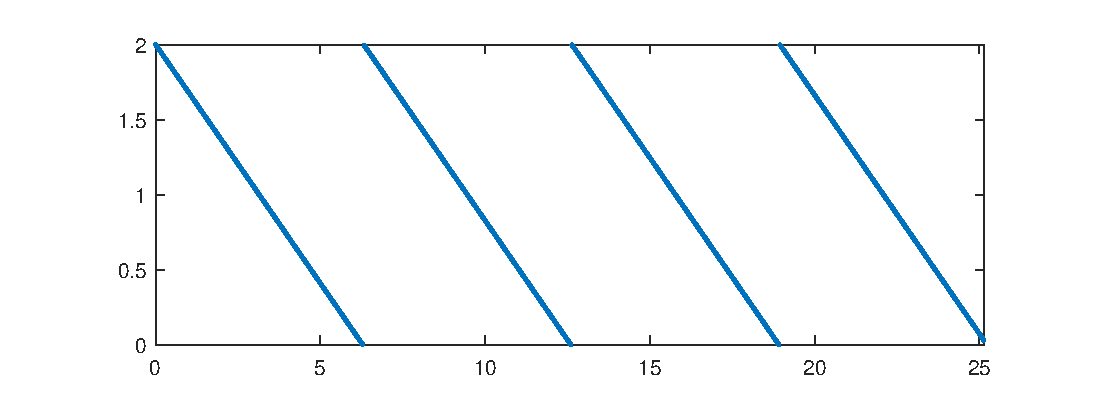
\includegraphics[scale=0.55]{smoothie.eps}}
\caption{Graf på hur mycket smoothie du har kvar!}
\label{}
\end{figure}
%TODO: Undvik \bf. Makrot heter \textbf sedan många år.
Grafen visar hur mycket som finns kvar medan du dricker och är periodisk eftersom du bara \textbf{måste} ha en till så fort smoothien är slut. Systemsvaret ska bara påverka frekvensen med jordgubb i. Därför utvecklar vi smoothien till en serie som innehåller alla dess frekvenser(ingredienser). Vi kan då hitta frekvensen som vi vill påverka och så vet vi också vilka vi vill låta bli att påverka. För att kunna göra den här uppdelningen så krävs följande formel:
\[ f(t) = \sum_{k=-1}^1 C_k e^{k j t} \]
där konstanten $C_k$ är given från:
\[C_k = \int_{k=-\infty}^{\infty} C_k e^{k j t}\]
För vår smoothie så kommer serien ha följande utseende:
\[f(t) = 2 \sum_{1}^{\infty} \frac{(-1)^{n+1}}{n} sin(n t) \]
Obs! \emph{Om vi istället valt att gå till kassan och bett om en ny smoothie, så hade vi alltså bytt insignal in i vårt system istället för att påverka den vi har.}
En mer matematiskt korrekt förklaring är att återigen observera den enkla signalen $sin(\omega_0 t)$. Som tidigare nämnt kan den skrivas om enligt Eulers formel till
\[ \frac{e^{j \omega_0 t} - e^{-j \omega_0 t}}{2j}\]
vilket kan skrivas som om vi låter $C_0=0$, $C_{1}=\frac{1}{2j}$ och $C_{1}=-\frac{1}{2j}$
\[ \sum_{k=-1}^1 C_k e^{j k \omega_0 t} \]
Låter vi nu även \textbf{alla} andra $C_k = 0$ förutom  $C_1$ och $C_{-1}$ blir formen
\[ \sum_{k=-\infty}^{\infty} C_k e^{j k \omega_0 t} \]
Det magiska är då att vi bara har skrivit om den ursprungliga funktionen, vilket innebär att
\[ \sin(\omega_0 t) = \sum_{k=-\infty}^{\infty} C_k e^{k j t} \]
%Funktionen behöver vara periodisk över någon konstant. Men det är mycket lättare att arbeta med 2pi.
%Om det är viktigt så kan vi låta dem applicera formeln
%$$ f(x) = \sum_{k=-1}^1 C_k e^{k j t} $$
%och $$C_k = \sum_{k=-\infty}^{\infty} C_k e^{k j t}$$
%Till sinus, och det kommer visa sig vara samma sak. Lämnas till en övning?
%Detta innebär att de måste lösa en Integral vilket inte använder sig av DSL...
%TODO: Som tidigare sagt: undvik \newline - använd en normal tomrad istället
Detta blir då en form av det som kallas för fourierserier. Man skriver om allt så att det uttrycks som komponenter till den hela signalen som man ''slår'' isär. Om man har en enkel signal som i vårt fall så är det kanske inte riktigt så givande, men om man har en större, mer komplicerad signal så skulle den vara svår att studera i sitt grundutförande och det skulle bli mycket lättare att bara bryta upp den till sina komponenter istället då.

%TODO: Det verkar vara ett ovanligt filter som tar bort "frekvenser som har en _amplitud_ större än ett visst tal \(K\)". Enkla filter brukar ta bort alla _frekvenser_ som är högre än en viss frekvens.
En fourierserie visar en amplitud mot dess frekvens, så man vet ''hur mycket'' bidrag man får från varje frekvens. Så ett ordentligt exempel skulle vara att man har ett filter som filtrerar bort alla frekvenser högre än en viss frekvens $K$. %som har en amplitud större än ett visst tal $K$.
Då kan man ta reda på vilka frekvenser som kommer att påverkas efter att filtret applicerats genom att bryta upp signalen till dess komponenter.

Detta är då användningsområdet för fourierserier i ett nötskal, inom signaler och system i alla fall. Det vill säga, bryta upp en signal i dess frekvenser för att finna mer information och tydligt kunna beräkna hur systemsvaret påverkar insignalen. Hur skulle det funka om insignalen inte var periodisk?

Det är där fouriertransformen kommer in!

\section{Fouriertransform}

Observera att signaler inte nödvändigtvis behöver vara periodiska. Hur ska man då kunna behandla dessa om en fourierserieutveckling kräver periodicitet? Vi transformerar dem! Om ni kommer ihåg att $e^{j\omega x}$ är en trigonometrisk funktion enligt Eulers formel. Då kanske följande formler blir logiska, och om de inte blir det så är det enda ni behöver veta att formlerna ''transformerar'' signalen så att den kan studeras i en frekvensdomän.

Definition för fouriertransform:
\[\hat{f}(\omega) = \int_{-\infty}^{\infty} f(t) e^{-j \omega t} dt\]

Vi kan sedan observera att det är samma sak som att beräkna ut konstanten $C_k$ men i detta fall så är $\omega_0$ en variabel istället för en konstant, vilken betecknas som $\omega$ för att visa skillnaden.
Detta kan användas inom matematiken för att beräkna differentialekvationer över begränsade tidsintervall. I princip så ändras det hela från ett tidsplan till ett frekvensplan, det vill säga att det ändras från linjer till cirklar. %Kanske är onödigt?
Bli nu inte skrämda av alla dessa integraler. Oftast så tillåts det en tabell som man kan använda sig av för att förenkla hela processen. Vi definerar en operator som fouriertransformerar $\mathcal{F}$. Några viktiga transformer:

%TODO: Lite oklart var t och \omega binds. Vänligen förklara att t binds (implicit) i vänsterledet (inom parentesen) och att \omega binds i högerledet (utanför parentesen).
\[\mathcal{F}(e^{j a t} f(t)) = F(\omega - a)\]%Translation
\[\mathcal{F}(f(at)) = \frac{1}{|a|}F(\frac{\omega}{a})\]%Skalning
\[\mathcal{F}(\frac{d}{dt} f(t)) = i\omega F(\omega) \]%Derivering

Fouriertransformen är även linjär vilket innebär
\[\mathcal{F}(a f + b g) = a F + b G\]

Om vi då återgår till vårt smoothie-exempel så skulle det vara som att vi låter en maskin hitta alla ingredienser i smoothien åt oss.

Varför skulle det här vara hjälpsamt? Om ni kommer ihåg från innan hur utsignalen till ett systemsvar är givet från $y(t) = x(t) * h(t)$, vilket är en faltning mellan två funktioner. I en frekvensdomän blir motsvarande $Y(\omega) = X(\omega) H(\omega)$. Det vill säga en enkel multiplikation mellan insignalen och \emph{frekvenssvaret} som är det fouriertransformerade impulssvaret.
\[\mathcal{F}(f*g) = F G \]

%Exempel på hur man fouriertransformerar i ett LTI-system.
\textbf{Exempel} %(inspirerad från en tenta uppgift) (Inte helt klar)
%OBS! Denna exempel använder sig av Invers Fourier Transform vilket vi introducerar efter.... så vi måste antingen dela upp exemplet eller flytta ner den. Cecilia får bestämma.
%OBS!! kanske för jobbig för ett exempel.
%OBS!!! Har ni lärt er en bättre metod för att hantera fourier transformen av en sinus? Detta är den enda metod jag kan. Vilket ger en trigonometrisk lösning skrivit i Eulers formel (tror jag). Skulle det vara ok att svara så i er tenta? Annars borde det gå att skriva om genom att multiplicera med nämnarens konjugat.

%TODO: kontinuerligt
Ett kontinuerligt LTI-system har insignalen $x(t)=\delta{t} + \cos(5 t)$ och impulssvaret $h(t) = e^{-2 t} u(t)$. Hur ser utsignalen ut?
\textbf{Lösning:}

Först beräknas fouriertransformen av impulssvaret ut.
\[\mathcal{F}(h) = H = \frac{1}{2+j \omega}\]
Eftersom fouriertransformen är linjär så kan vi behandla termerna i insignalen var för sig. Det vill säga
\[\mathcal{F} (x) = \mathcal{F}(\delta{t}) + \mathcal{F}(\cos(5 t) = X_1 + X_2 \]
Som båda är givna från tabeller och blir $1+\pi(\delta(\omega - 5) + \delta(\omega + 5))$. Vi har nu tagit bort faltningen och har följande förhållande.
\[Y = X H = X_1 H + X_2 H\]
Vilket innebär att vi har löst problemet om vi återtransformerar vänsterledet. Vi börjar med $X_1 H$
\[y_1=\mathcal{F}^{-1}(X_1 H) =  \int_{-\infty}^{\infty} 1 \cdot \frac{1}{2+j \omega} e^{j \omega t} d\omega = e^{2 t} u(-t)\]
Nu återstår bara $X_2 H$
\[y_2=\mathcal{F}^{-1}(X_2 H) = \int_{-\infty}^{\infty} \pi(\delta(\omega - 5) + \delta(\omega + 5)) \cdot \frac{1}{2+j \omega} e^{j \omega t} d\omega \]
%TODO: Det vore bra att vara mer tydlig här: vad innebär "knasig" och vilken definition hänvisas till?
Integralen ovan innehåller impulsfunktioner vilket gör den svår att förstå intuitivt. Om man kollar på impulsfunktionens definition

\[
\delta(\omega - \tau)=
\begin{cases}
"\infty",\quad \omega = \tau \\
0, \quad else
\end{cases}, \omega \in \mathbb{R}
\]

så ser vi att integranden bara kan anta värden då $\omega=5$ eller $\omega =-5$ eftersom annars tar impulsfunktionen värdet 0. Detta innebär att integralen blir följande:
\[\frac{1}{2+j 5} e^{j 5 t} + \frac{1}{2-j 5} e^{-j 5 t}\] %Som förmodligen kan skrivas om till andra trigonometriska funktioner. Ska jag göra det?
Utsignalen blir då $y=y_1 + y_2$ eller $e^{2 t} u(-t) + \frac{1}{2+j 5} e^{j 5 t} + \frac{1}{2-j 5} e^{-j 5 t}$
%---------------------------------Slut på exempel-----------------------

Sen finns även Plancherel's ekvation: %Parsevals
%$$ 2 \pi <f,f> = <F,F> $$
%$$<f,f> = \int_{-\infty}^{\infty} |f(x)|^2 dx $$
\[\int_{-\infty}^{\infty} |f(x)|^2 dx = \frac{1}{2 \pi}\int_{-\infty}^{\infty} |F(\omega)|^2 d\omega \] %Enligt Beta s.316, säger i princip samma sak men kanske är tydligare. Kan ta bort den ovan.

Det vill säga normen av en funktion är samma sak som normen av dess fouriertransform delat med $2 \pi$. Eller mer specifikt, delat med perioden som den är definierad över. Inom detta området innebär normen av en signal den totala energin av signalen. %Vettigt när man kollar på totala energin i en signal. Exempel är nice!

\textbf{Exempel}
Vi vill veta den totala energin i insignalen till ett system givet utsignalen y och impulssvaret h. Fouriertransformerar vi systemet får vi
\[XH = Y \implies X = Y/H\]
Detta ger oss enligt Plancherels formel följande relation
\[ \frac{1}{2 \pi} \int_{-\infty}^{\infty} |X(\omega)|^2 d \omega = \int_{-\infty}^{\infty} |x(t)|^2 d t \]
Där vi kan se att högerledet är den totala energin från insignalen.
Det vill säga, bara lös vänsterledet.

Så varför använda fouriertransform? I detta fall finns det två anledningar. %Kanske mer?

Det kan vara svårt att bryta upp en faltning! (Det vill säga vi vill bryta upp $x*h=y$ så att x blir ensam.)

Så varför använda Plancherels sats? Mycket lättare att slippa återtransformera och sedan beräkna normen. (Det vill säga högerledet...)
%Vad finns kvar att göra, komma på en utsignal och impulssvar som gör följande integral enkel $\int_{-\infty}^{\infty} |(Y/H)(\omega)|^2 d \omega$
%Såvida det här inte räcker.
%--------------------------Slut på Exempel----------------------------

\textbf{OBS!} Tillskillnad från när man utvecklar signalen till dess fourierserie så är en transformerad funktion \textbf{inte} samma sak som den ursprungliga funktionen. Därför önskas det att återtransformera funktionen, vilket görs med följande formel!

Invers fouriertransform -
\[f(t) = \frac{1}{2 \pi} \int_{-\infty}^{\infty}  e^{j \omega t} d\omega \]

Allt detta är under antagandet att signalens funktion är känd. Vad händer då om bara signalens värden är kända?

%I princip, fouriertransform används på signaler som är periodiska eller definierad i [-\infty,\infty]. Laplace på LTI system för system definierade från 0 till \infty (anses oftast vara enklare att behandlar en Fourier). Z-transform används på talserier ekvationer (differensekvationer).
\section{Diskret Fourier Transform}
%Vi borde kanske förklara sampling tydligare någon stans? Eller räcker detta? Mer är alltid bra. Dyker ändå upp på tentor.
%TODO: Ja - sampling är en central operation (och också linjär, tar funktioner till funktioner, etc.)
%Från det jag hittar så är sampling att reducera en kontinuerlig signal till diskret...
%Detta kan göras genom att ta värden i jämna interval från en signal.

Innan vi börjar med diskret fourier transform så förklarar vi lite om det viktiga begreppet \emph{sampling.}
%Om detta är inte tillräckligt kan jag ta med samplingteoremet och förklara det. Samplingstheoremet är jättebra att ta med!
%Jag kan också skapa en bild likt den i wikipedia om ni tycker att det behövs.

Sampling är definierad som \emph{genereringen av en ordningsföljd från en kontinuerlig insignal $x(t)$}. Vi får alltså talföljden $x(t_1), x(t_2), x(t_3)... $, där $t_n$ är tidpunkterna vi samplade. Vi låter nu denna talföljd skrivas om som $x[n]$, där n är värdets ordning i talföljden. Vi kan alltså se det som en funktion:

%-Visa upp det kodmässigt på något sätt?
%\begin{minted}[haskell]

%\end{minted}

Med andra ord, med hjälp av sampling kan vi reducera en kontinuerlig signal till en diskret signal. Därefter kan vi använda definitionen för DFT, \emph{diskret fouriertransform}, för att omvandla signalen från en tidsdomän till en frekvensdomän.
\[X[k] = \frac{1}{N} \sum_{n=0}^{N-1} x[n] e^{-2 \pi j n k/N}\]
Det vill säga, om man vill studera diskreta värden från en signal i dess frekvensdomän, då applicerar man DFT! Och precis som i det kontinuerliga fallet så finns det en invers DFT för att återomvandla signalen.
\[x[n] = \sum_{k=0}^{N-1} X[k] e^{2 \pi j n k/N} \] %Betas
%$$x[n] = \frac{1}{2\pi} \int X[k] e^{j n k}$$ TSS bokens definition
Rent praktiskt används diskret fouriertransform oftast med sampling från en typ av signal. Detta görs ifall det finns någon typ av okänd signal, där vi känner till \textbf{värden} men inte själva \textbf{formeln}. %Kom ihåg att rätta mig ifall jag har fel.
Här är även det motsvarande Parsevals ekvation

Parsevals ekvation för diskreta Fouriertransformer
%$$\sum_{-\infty}^{\infty} |x[n]|^2 = \frac{1}{2\pi} \int_{\pi}|X(\omega)|^2 d\omega $$
%TSS bokens definition.

\[\sum_{n=0}^{N} |x[n]|^2 = \frac{1}{N} sum_{k=0}^{N-1} |X[k]|^2 \]
%Wikipedias vilket är den jag känner till.

%Hur visar man exemplar på diskret fourier transform? Oftast brukar de användas numerisk väl? Lämnas som diskussion till gruppen.


\end{document}
